% Created with jtex v.1.0.21
\documentclass[a4paper,11pt,oneside]{book}
\usepackage[top=2cm, bottom=2cm, left=2cm, right=2cm]{geometry}
\usepackage[T1]{fontenc}
\usepackage[utf8]{inputenc}
\usepackage{lmodern}
\usepackage{graphicx}
\usepackage{caption}
\usepackage{natbib}
\usepackage{xcolor}
\usepackage{changepage}
\usepackage{framed}
\usepackage{hyperref}
\usepackage{amssymb}
\usepackage{float}
\usepackage{placeins}
\bibliographystyle{abbrvnat}

% Force figures to stay where declared
\floatplacement{figure}{H}

% Caption styling: small font, justified
\captionsetup{font=small, justification=justified, singlelinecheck=false}

% Make list items more compact
\usepackage{enumitem}
\setlist[itemize]{noitemsep, topsep=0pt}

%%%%%%%%%%%%%%%%%%%%%%%%%%%%%%%%%%%%%%%%%%%%%%%%%%
%%%%%%%%%%%%%%%%%%%%  imports  %%%%%%%%%%%%%%%%%%%
\usepackage{amsmath}
\usepackage{graphicx}
%%%%%%%%%%%%%%%%%%%%%%%%%%%%%%%%%%%%%%%%%%%%%%%%%%


\hypersetup{
  colorlinks,
  linkcolor={black},
  citecolor={black},
  urlcolor={black}
}

% Style quotes
\definecolor{darkblue}{rgb}{0.0, 0.0, 0.55}
\definecolor{quoteshade}{rgb}{0.95, 0.95, 1}
\renewenvironment{quote}{%
  \def\FrameCommand{%
    \hspace{1pt}%
    {\color{darkblue}\vrule width 2pt}%
    {\color{quoteshade}\vrule width 4pt}%
    \colorbox{quoteshade}%
  }%
  \MakeFramed {\advance\hsize-\width \FrameRestore}%
  \noindent\hspace{-8pt}% disable indenting first paragraph
  \begin{adjustwidth}{0pt}{0pt}% adjust as needed
  \vspace{2pt}\vspace{2pt}%
}
{%
  \vspace{2pt}\end{adjustwidth}\endMakeFramed%
}

\title{\Huge \textbf{Supplementary Figures}}
\author{\textsc{}}

\begin{document}
\sloppy

\frontmatter
\maketitle

\tableofcontents
% \listoffigures
% \listoftables

\mainmatter

\begin{verbatim}
<IPython.core.display.Markdown object>
\end{verbatim}


\clearpage
\begin{figure}[!htbp]
\centering
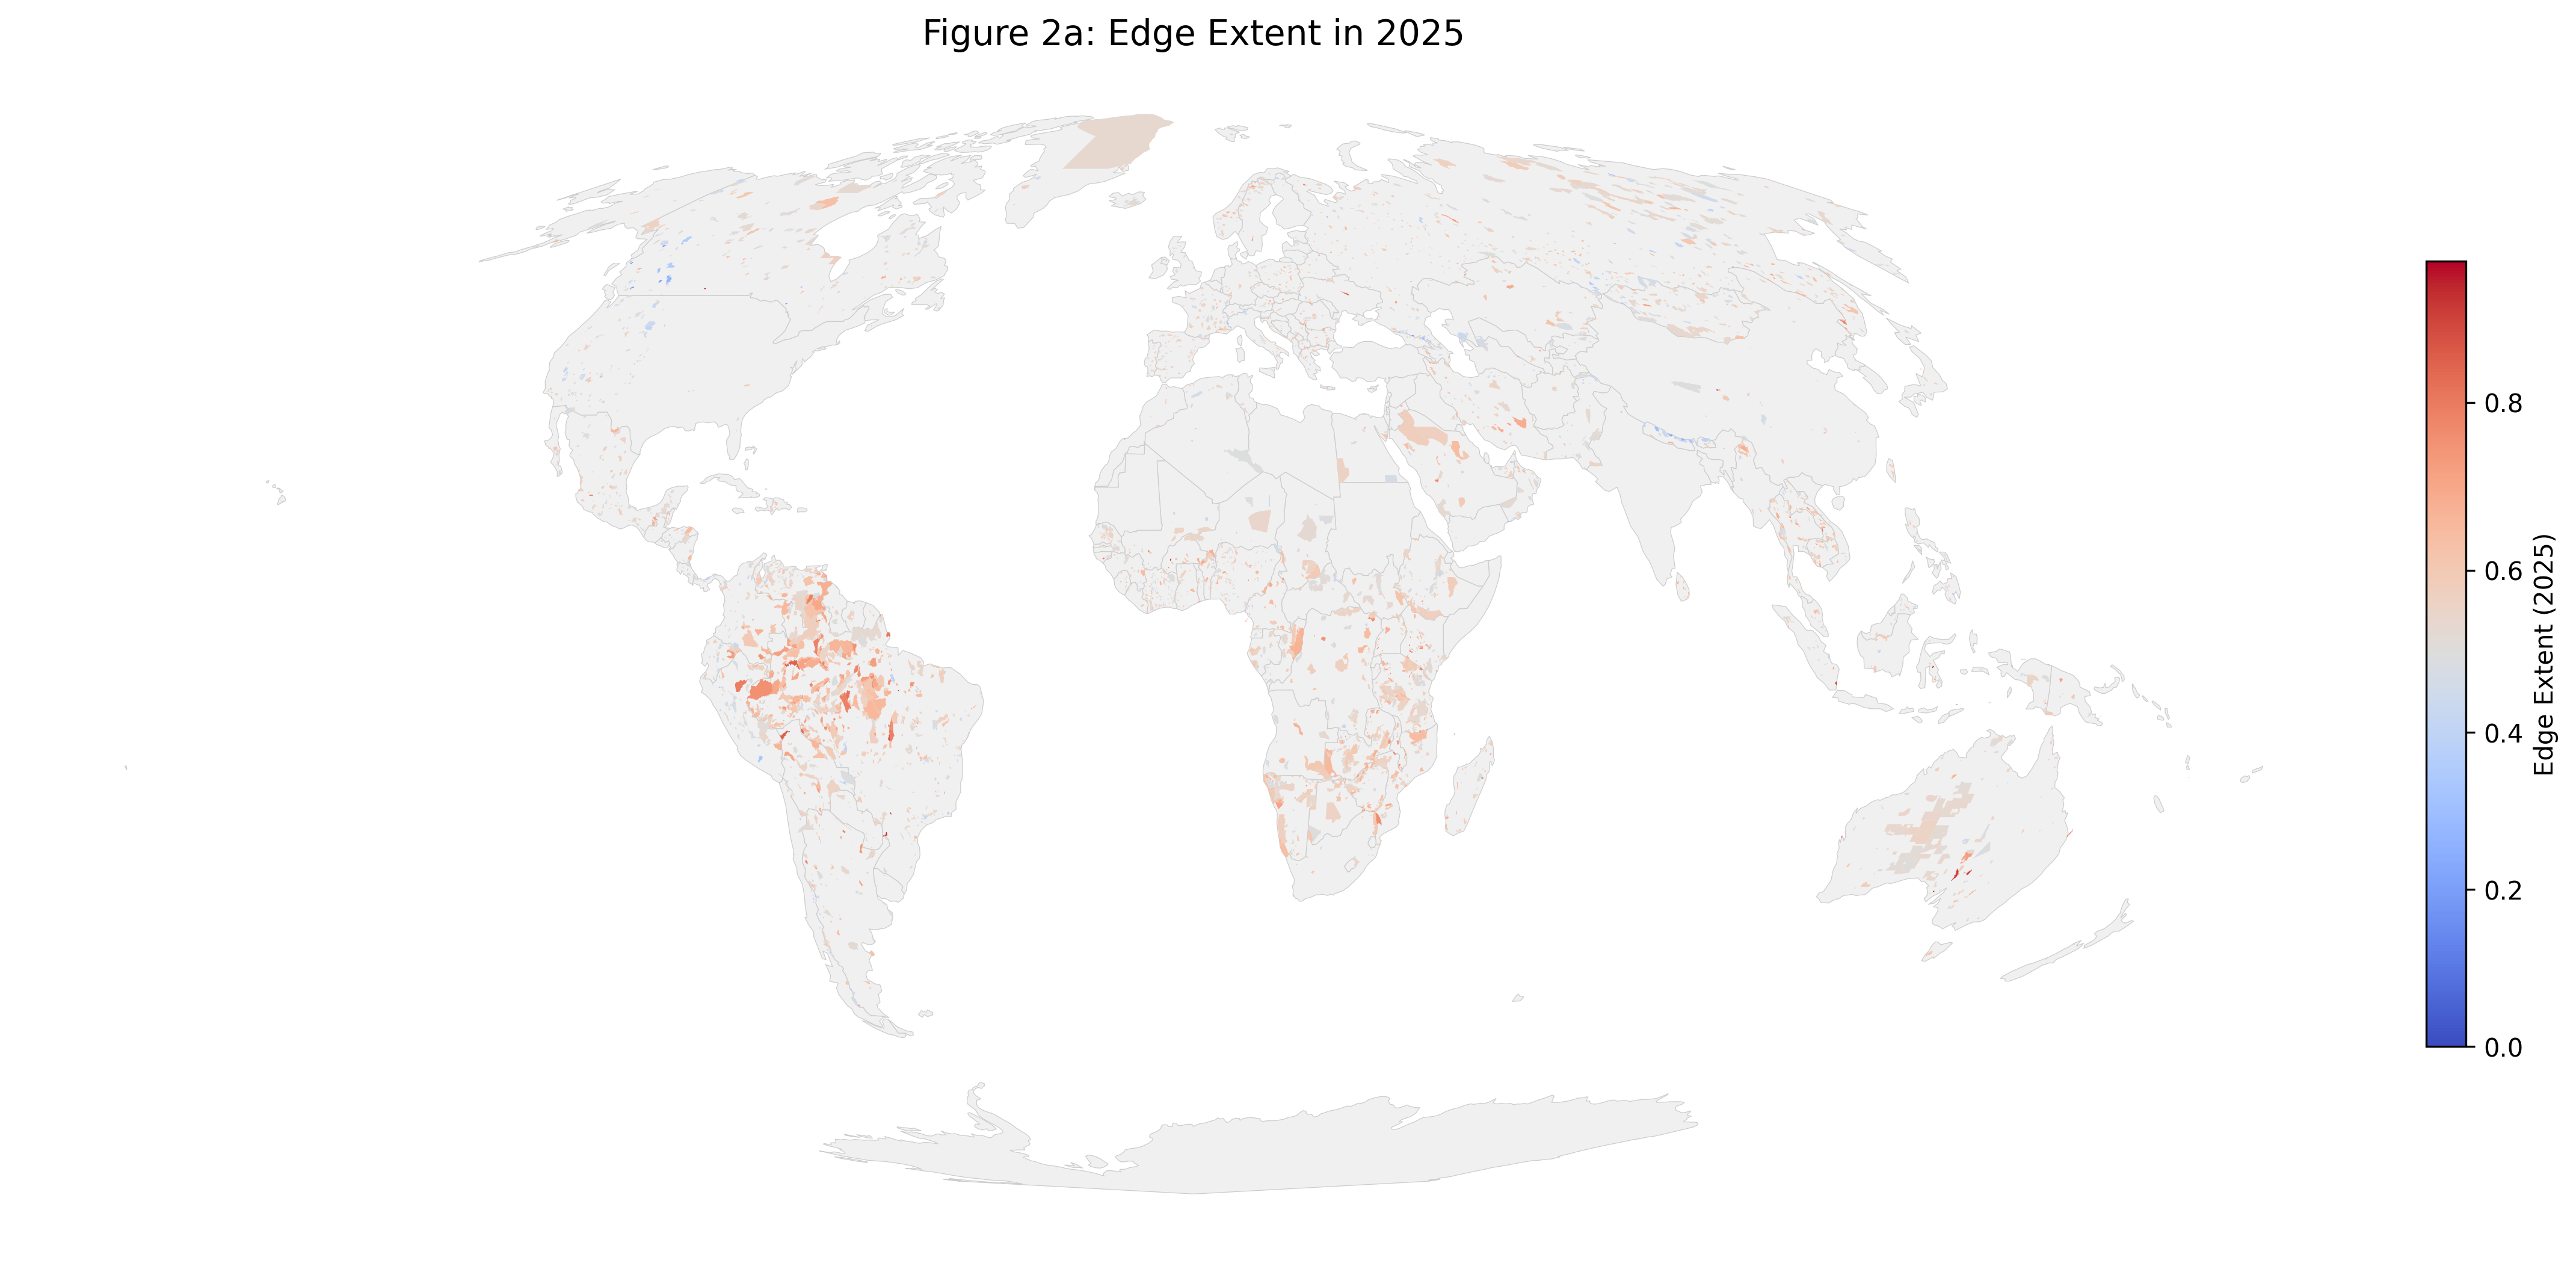
\includegraphics[width=1\linewidth]{files/ndvi_figure2a_extent-1f0028db577f6d9b28894911d398d140.png}
\end{figure}

\begin{figure}[!htbp]
\centering
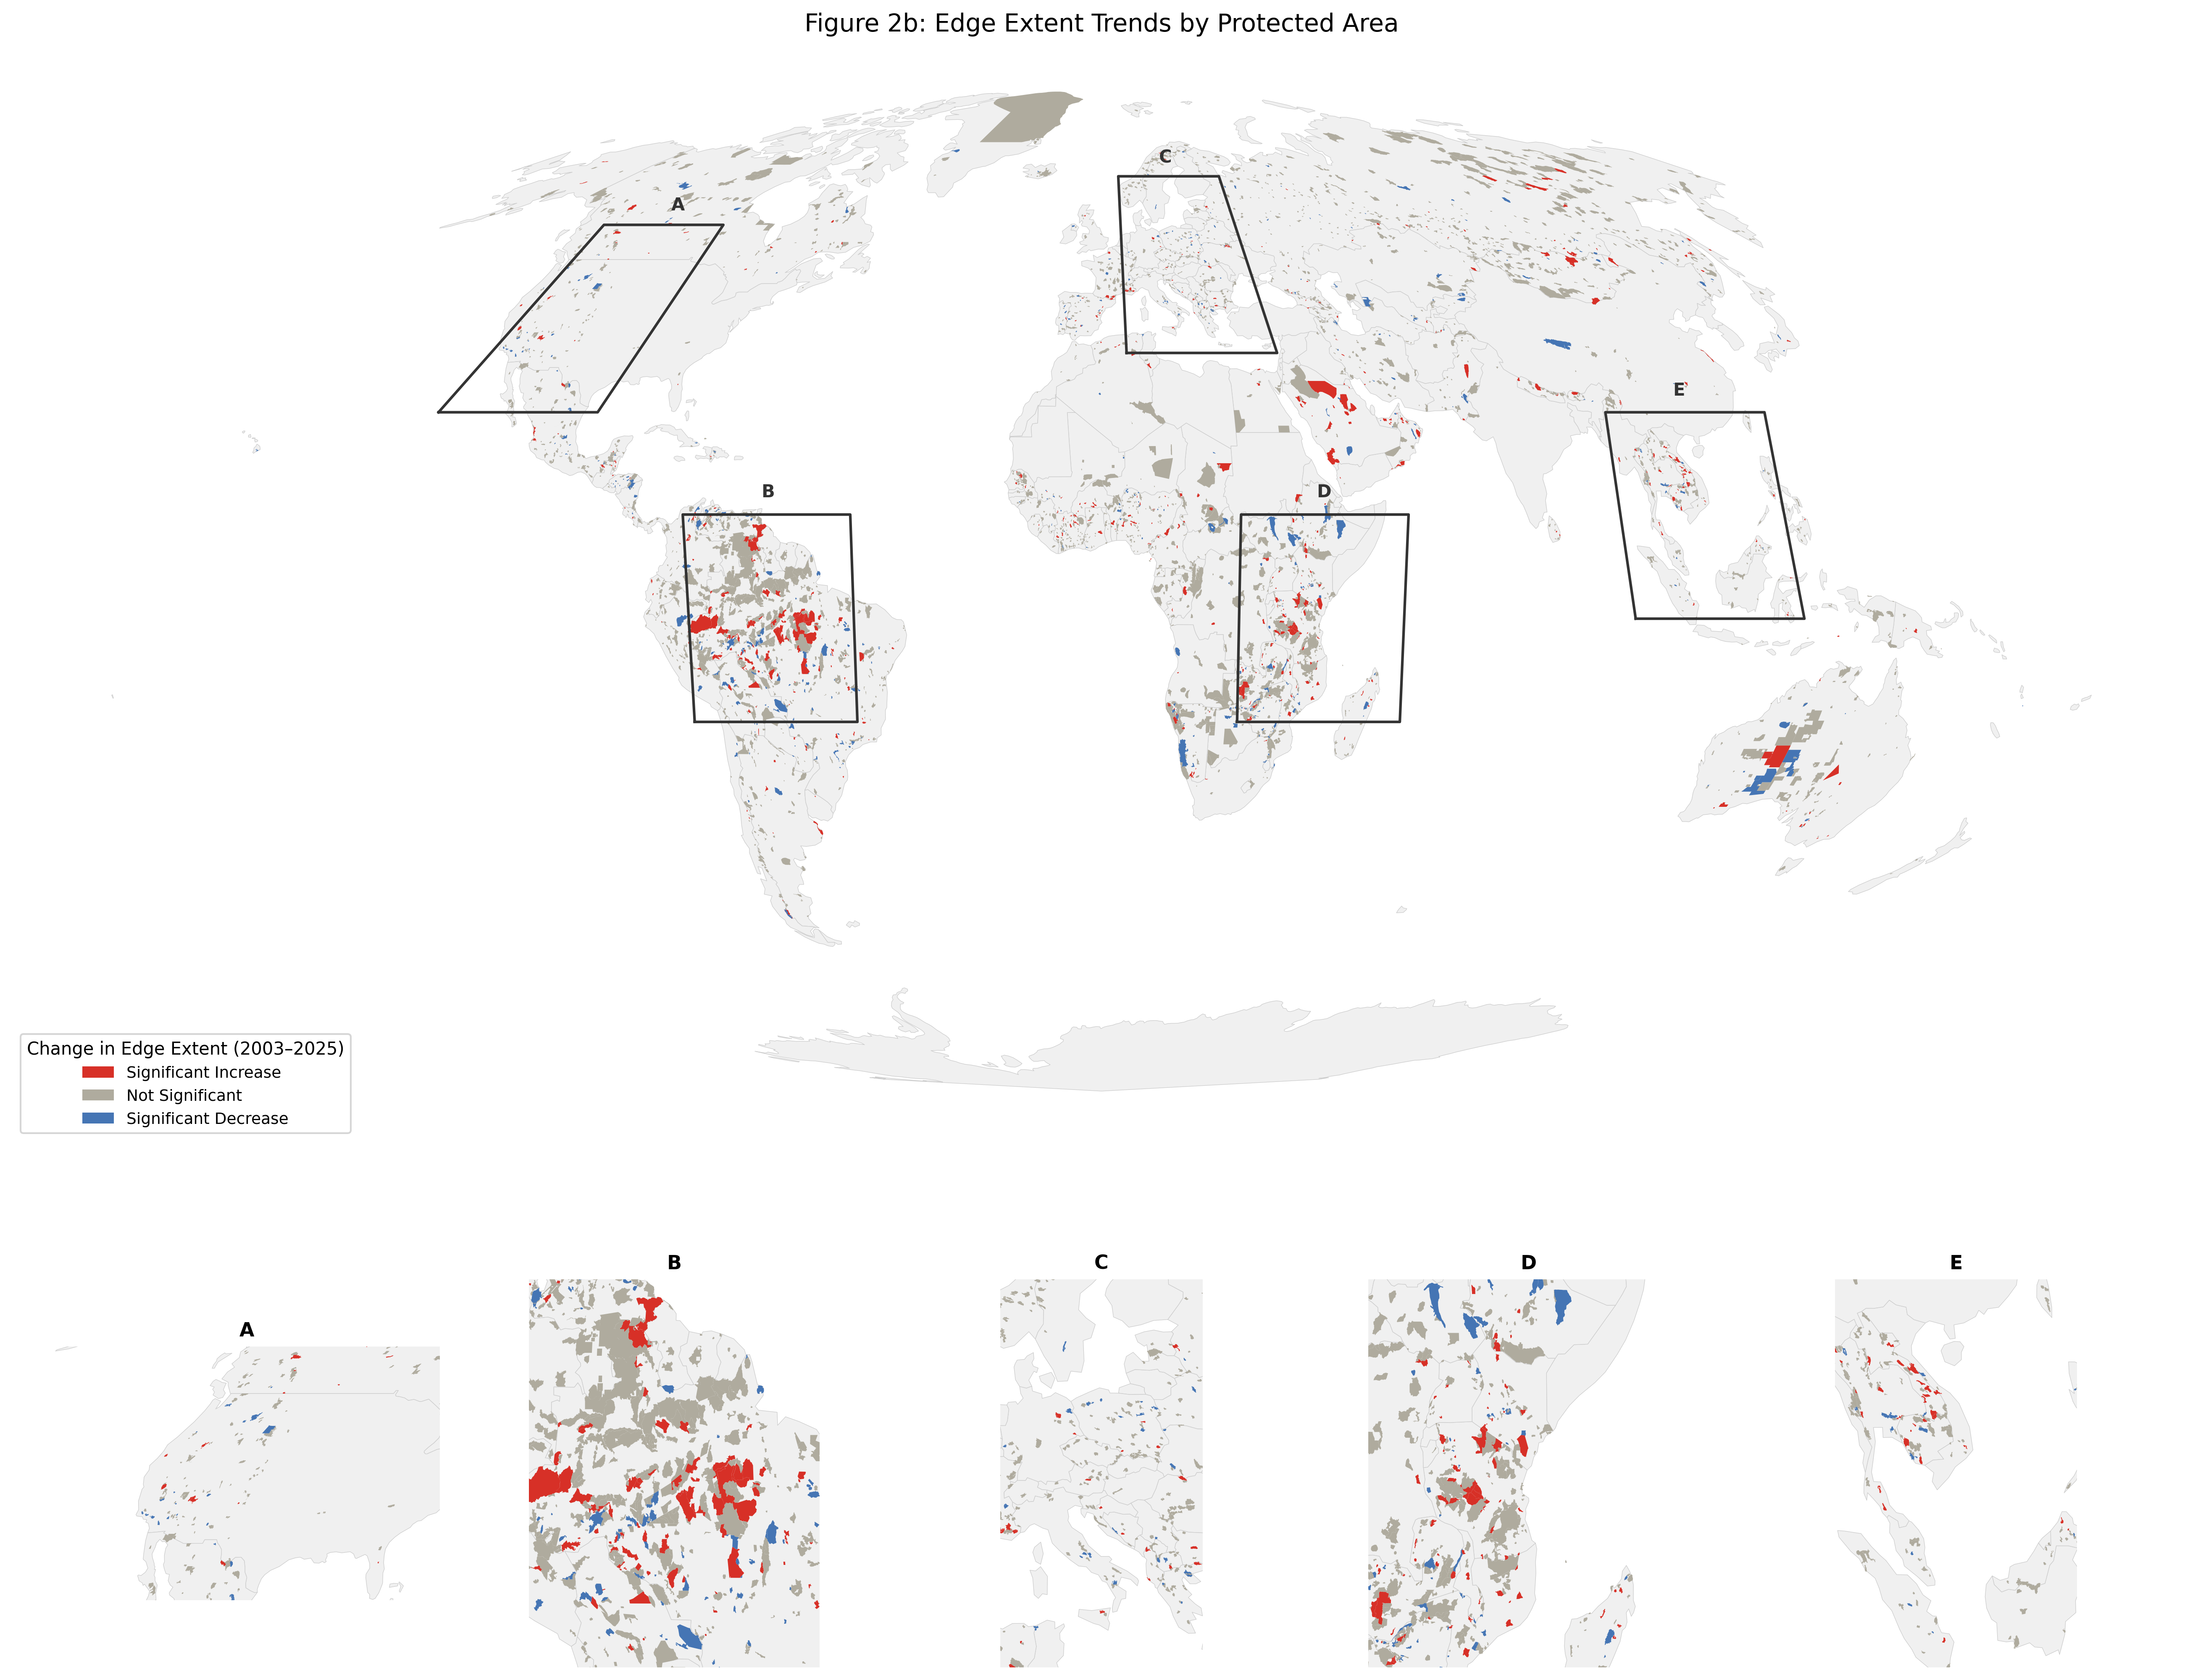
\includegraphics[width=1\linewidth]{files/ndvi_figure2b_trend_-795651c115d0ad42b89bcd00f894762a.png}
\end{figure}


{\small \noindent \textbf{Figure 2.} (a) Spatial distribution of edge extent across protected areas in 2025. (b) Significant temporal trends in edge extent (2003--2025); red = significant increase, blue = significant decrease, grey = not significant.}

\vspace{1em}
Edge extent varies widely across regions, with tropical and grassland PAs tending toward higher values. Significant increases cluster in sub-Saharan Africa and South America, while significant decreases are concentrated in boreal and temperate zones.


\clearpage
\begin{figure}[!htbp]
\centering
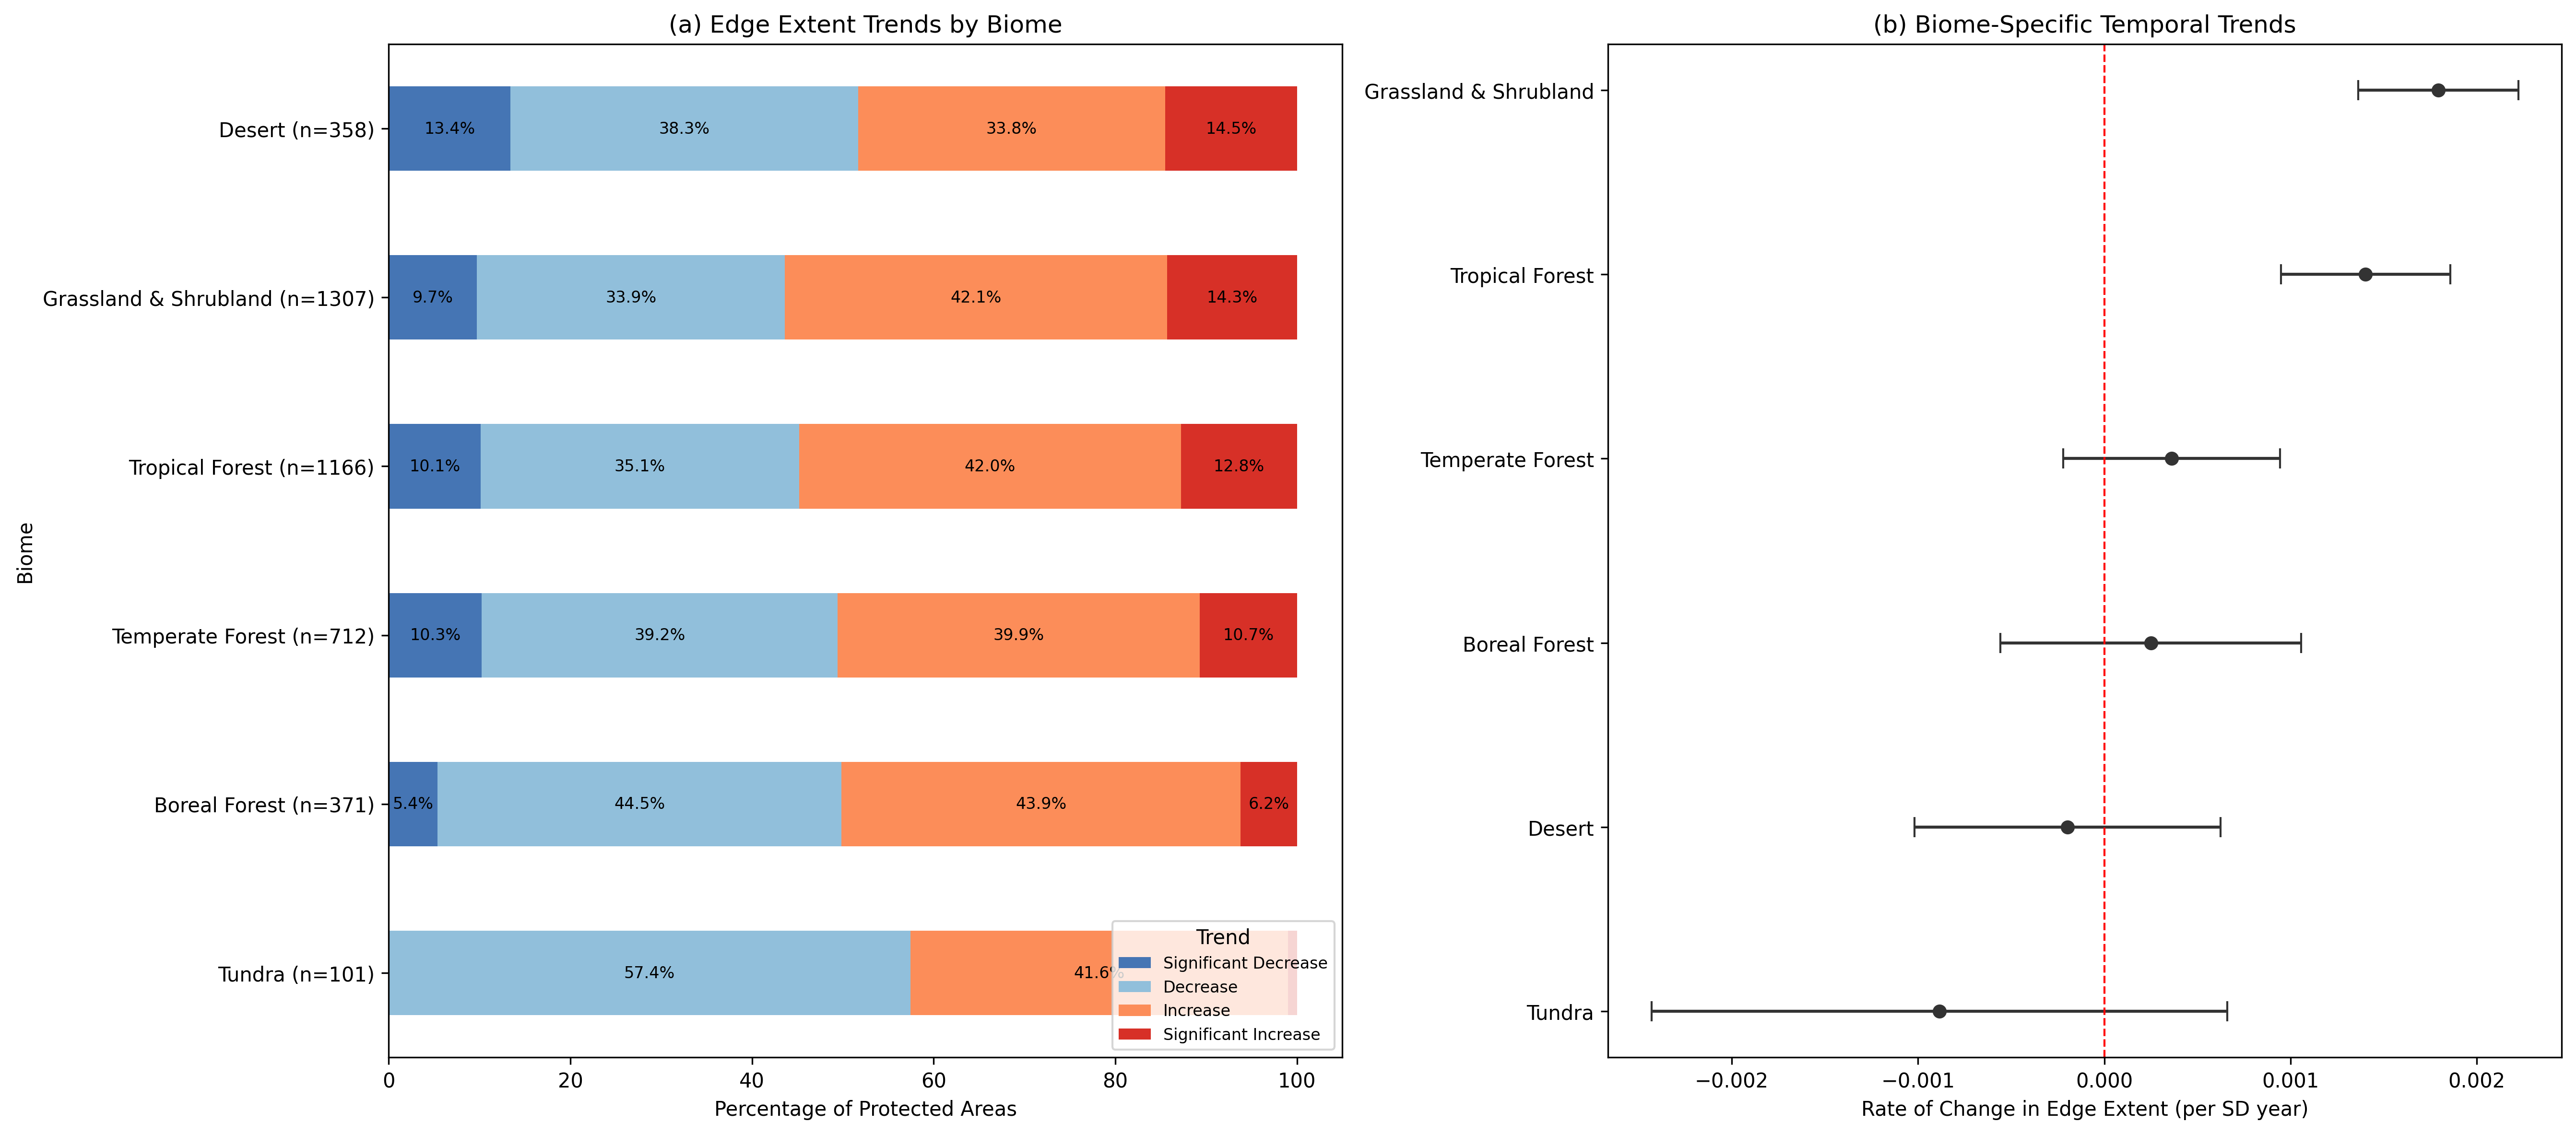
\includegraphics[width=1\linewidth]{files/ndvi_figure3_trends_-c9d73d32a539dda07f9a208103d4c357.png}
\end{figure}


{\small \noindent \textbf{Figure 3.} (a) Proportion of PAs per biome classified by edge-extent trend direction and significance. (b) Biome-specific rates of change in edge extent (slope per SD-year) from the mixed-effects trend model with 95\% confidence intervals.}

\vspace{1em}
Biome-specific temporal trends were estimated using a linear mixed-effects model:

\begin{equation}
\text{edge\_extent}_{ij} = \beta_0 + \beta_1 \, \text{year}_z + \boldsymbol{\beta}_2 \, \text{Biome}_i + \boldsymbol{\beta}_3 \, (\text{year}_z \times \text{Biome}_i) + u_j + \varepsilon_{ij}
\end{equation}

where $u_j \sim \mathcal{N}(0, \sigma_u^2)$ is a random intercept for PA $j$. Grassland \& Shrubland and Tropical Forest biomes show significant positive temporal trends in edge extent.


\clearpage
\begin{figure}[!htbp]
\centering
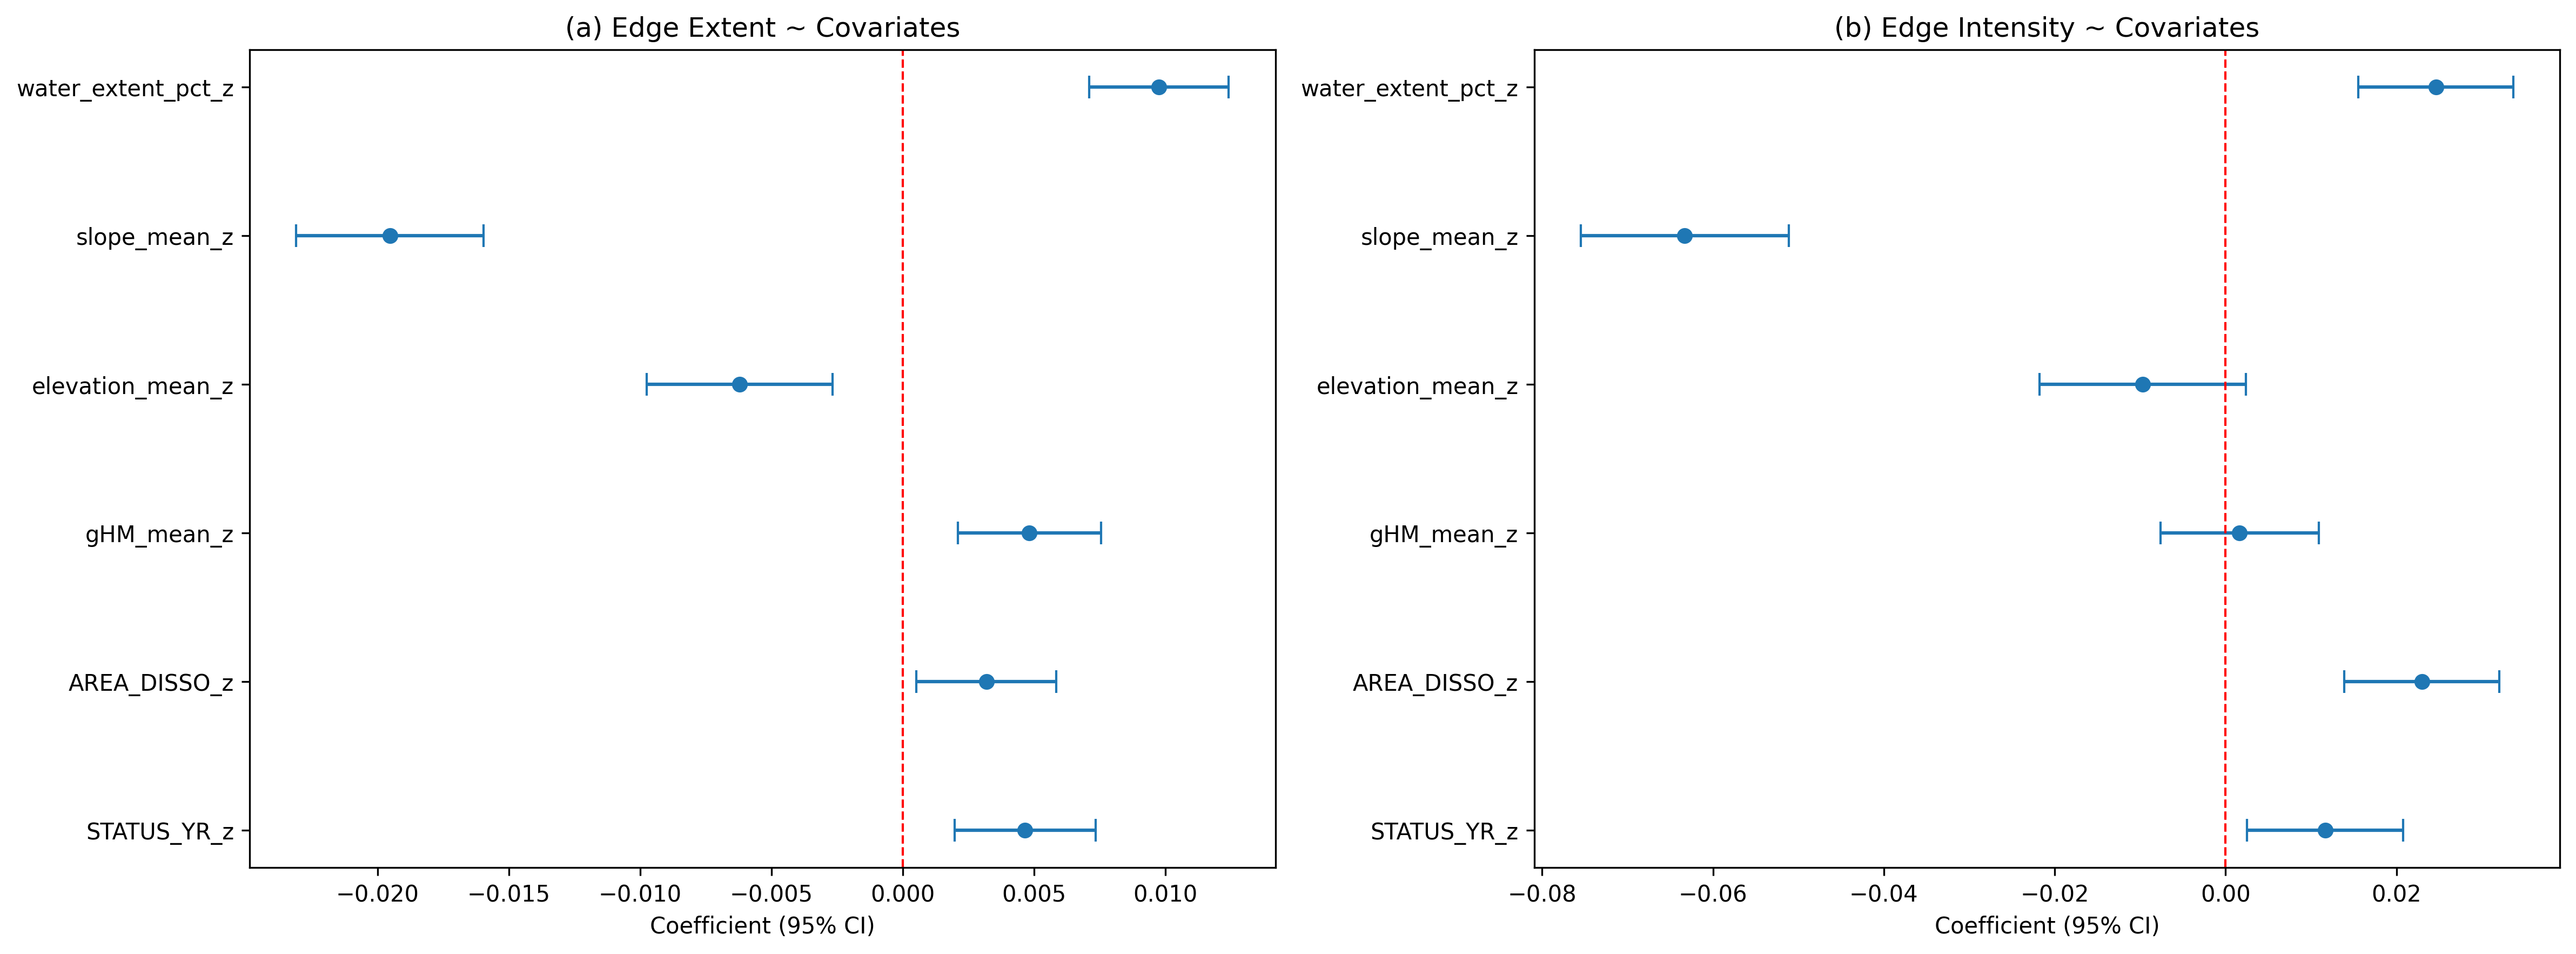
\includegraphics[width=1\linewidth]{files/ndvi_figure4_mixed_m-8250225ca0eddb18e7faa69e9b308a27.png}
\end{figure}


{\small \noindent \textbf{Figure 4.} (a) Standardised mixed-model coefficients for edge extent in 2025. (b) Standardised mixed-model coefficients for edge intensity in 2025. Error bars denote 95\% confidence intervals; the dashed red line marks zero.}

\vspace{1em}
Cross-sectional drivers of edge effects in 2025 were assessed using linear mixed-effects models of the form:

\begin{equation}
y_j = \beta_0 + \sum_{k} \beta_k \, x_{kj}^{(z)} + u_j + \varepsilon_j
\end{equation}

where $y$ is edge extent or edge intensity, $x_k^{(z)}$ are z-scored covariates (status year, PA area, gHM, elevation, slope, water extent), and $u_j \sim \mathcal{N}(0, \sigma_u^2)$. Lower slope and elevation are related to higher edge extent and intensity, while higher water extent and human modification (gHM) outside of the park are associated with higher edge extent and intensity. PA area has a small but significant positive effect on edge intensity.


\clearpage
\begin{figure}[!htbp]
\centering
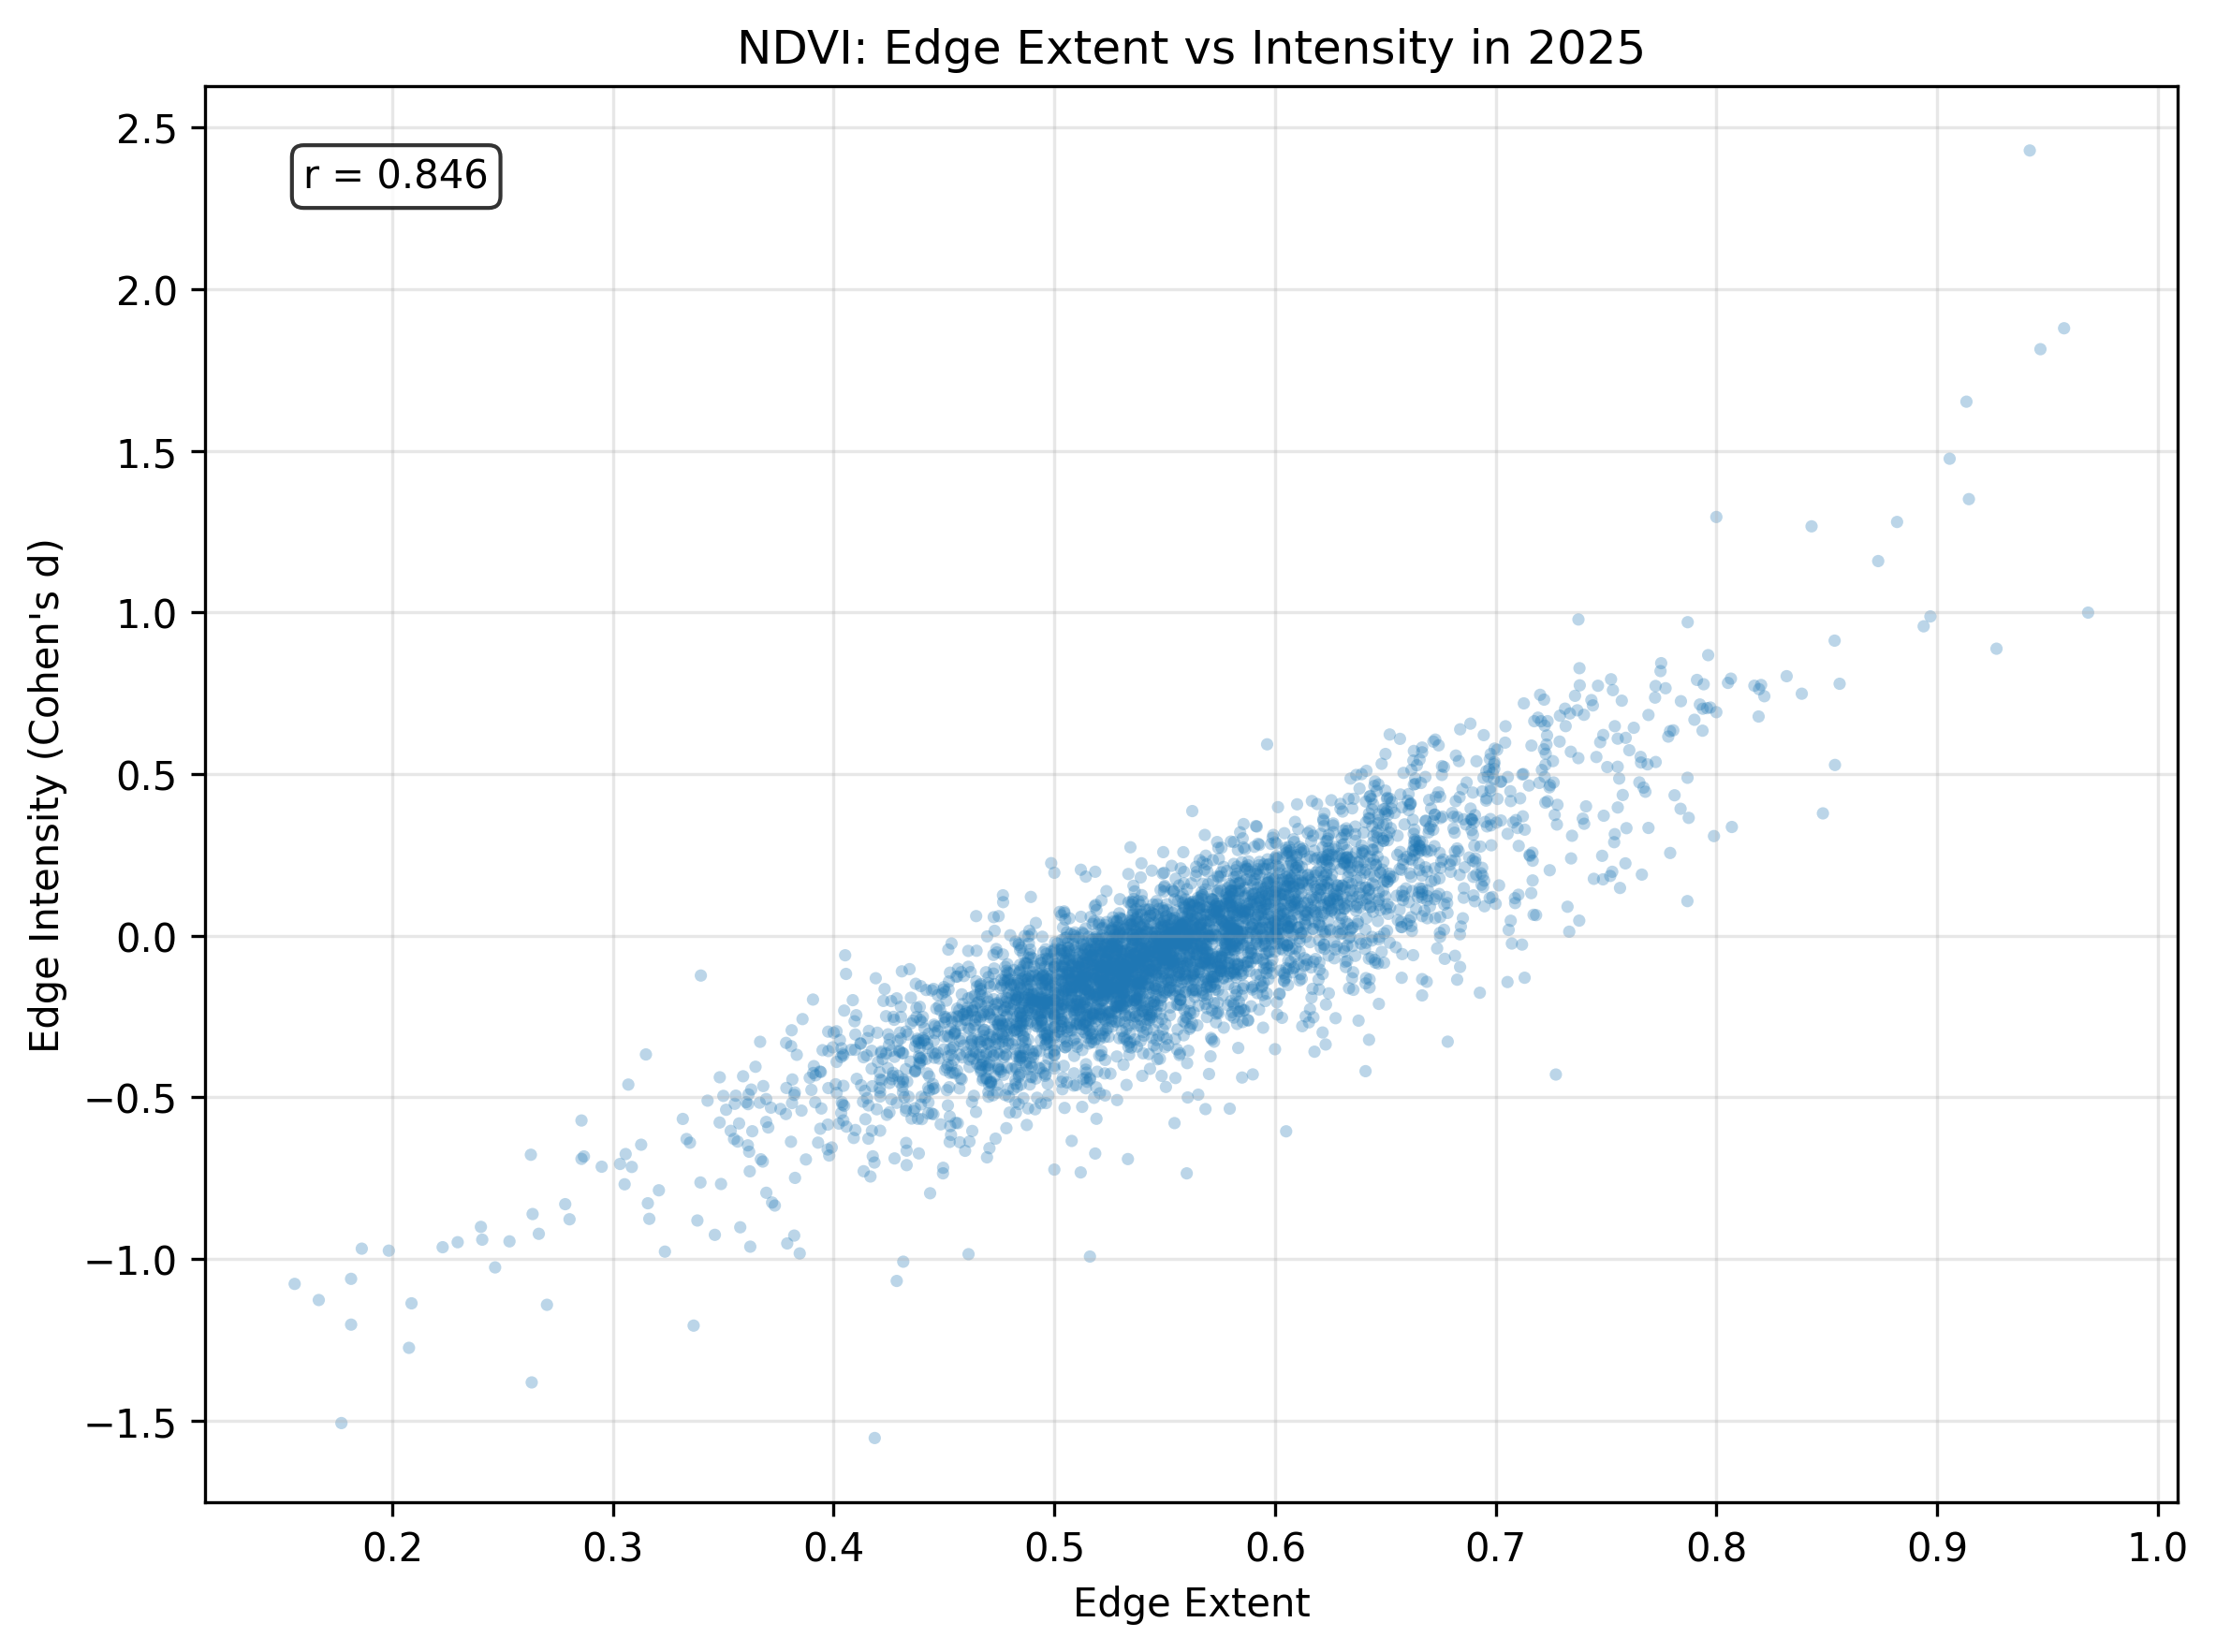
\includegraphics[width=1\linewidth]{files/ndvi_figure5a_correl-fac5fa6cd9043b27d805e7139360ad2e.png}
\end{figure}

\begin{figure}[!htbp]
\centering
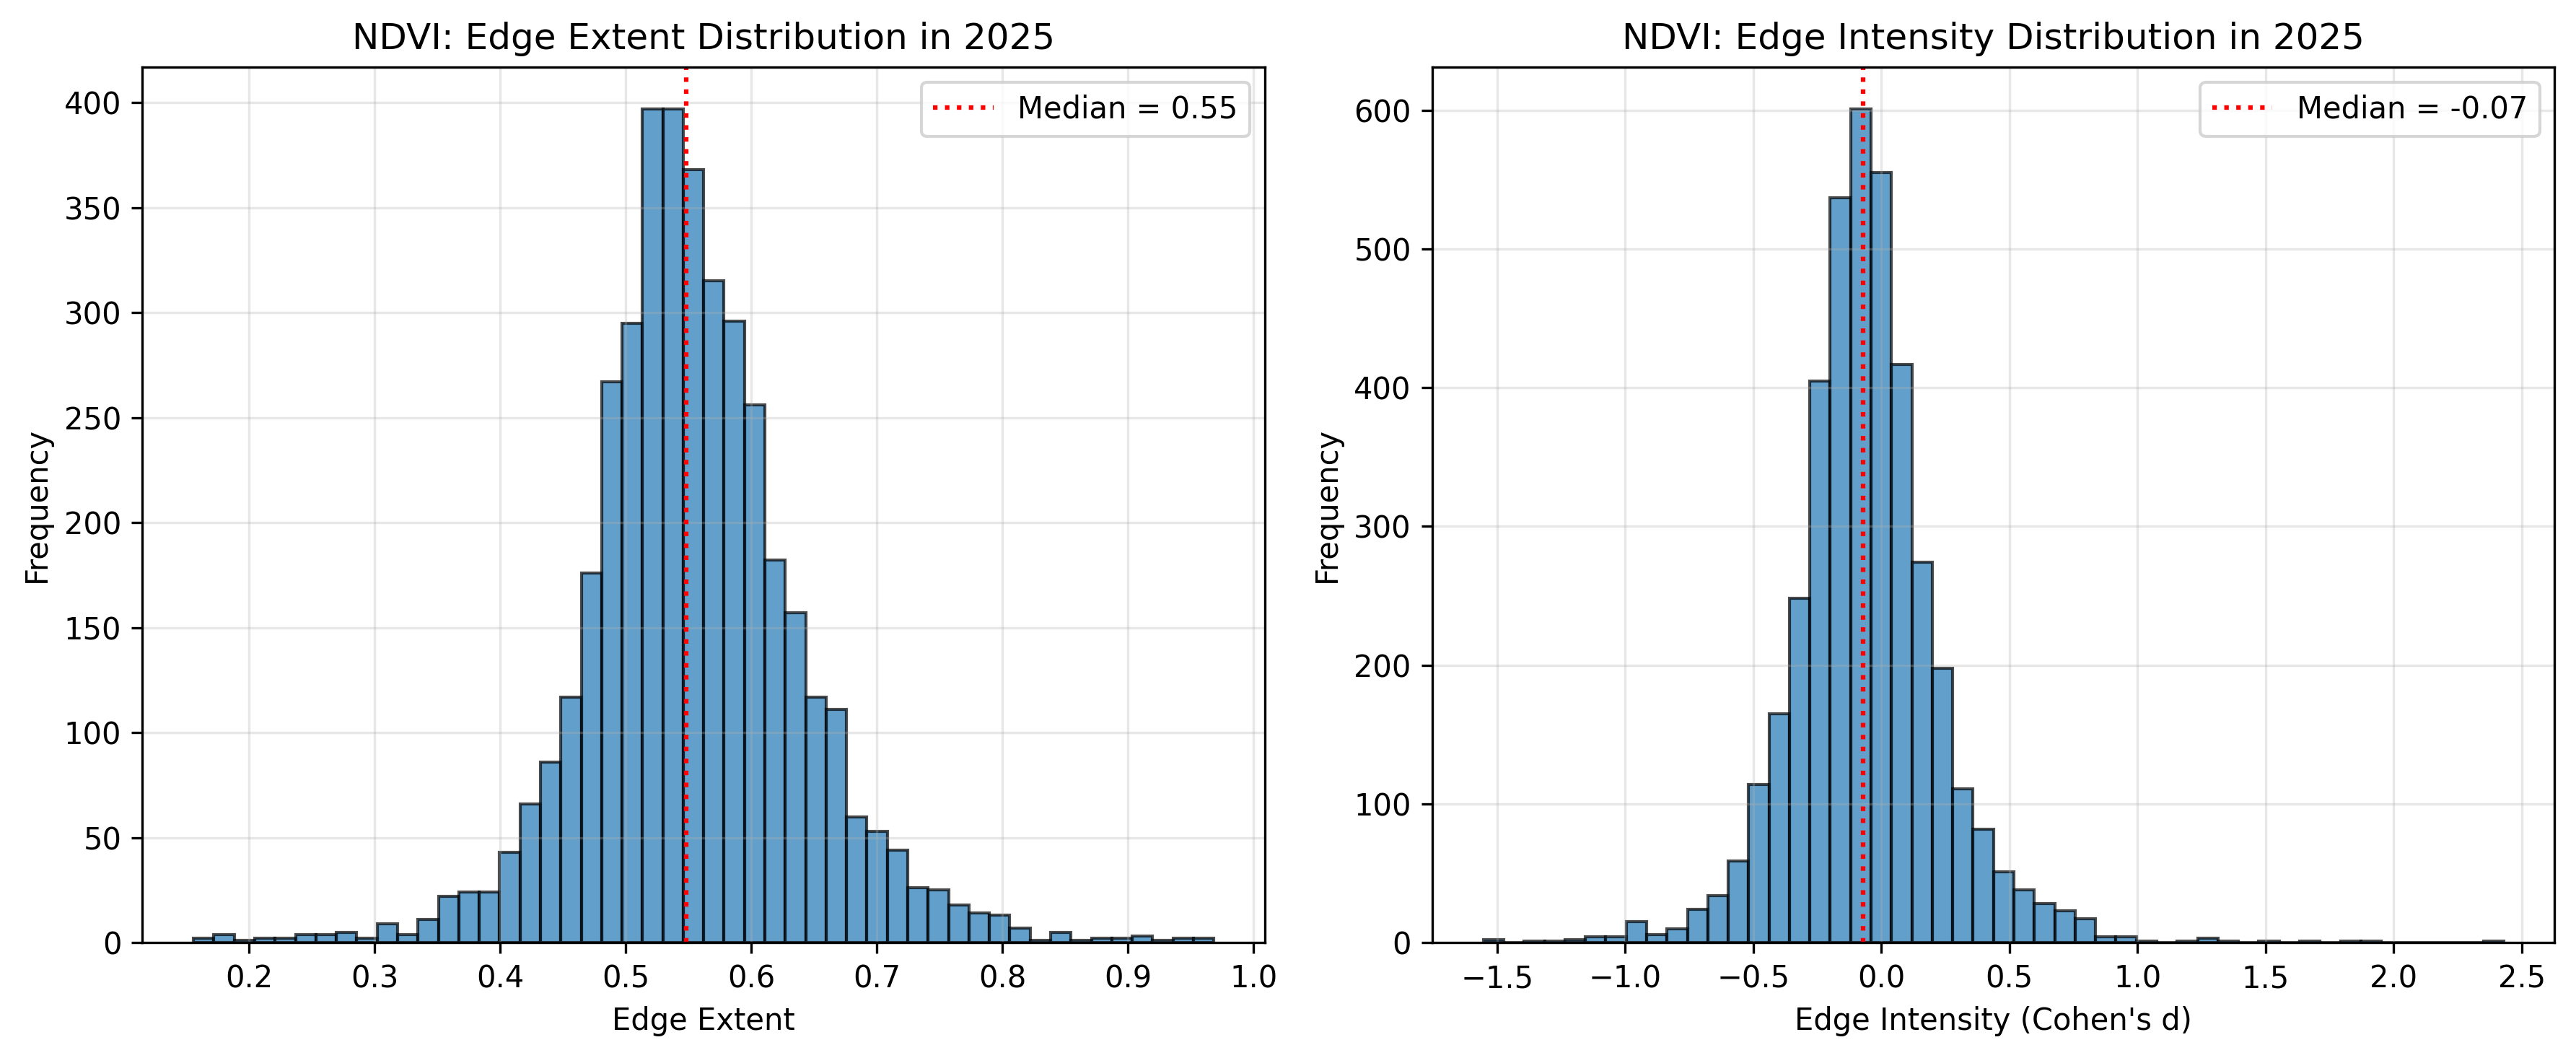
\includegraphics[width=1\linewidth]{files/ndvi_figure5b_distri-8bb8eaf02e04c815b979279f0abfe36a.png}
\end{figure}


{\small \noindent \textbf{Figure 5.} (a) Scatter plot of edge extent versus edge intensity (Cohen's d) for all PAs in 2025. (b) Distributions of edge extent and edge intensity across all PAs.}

\vspace{1em}
Edge extent and intensity are positively correlated, with a saturation effect apparent in the highest values.


\clearpage
\begin{figure}[!htbp]
\centering
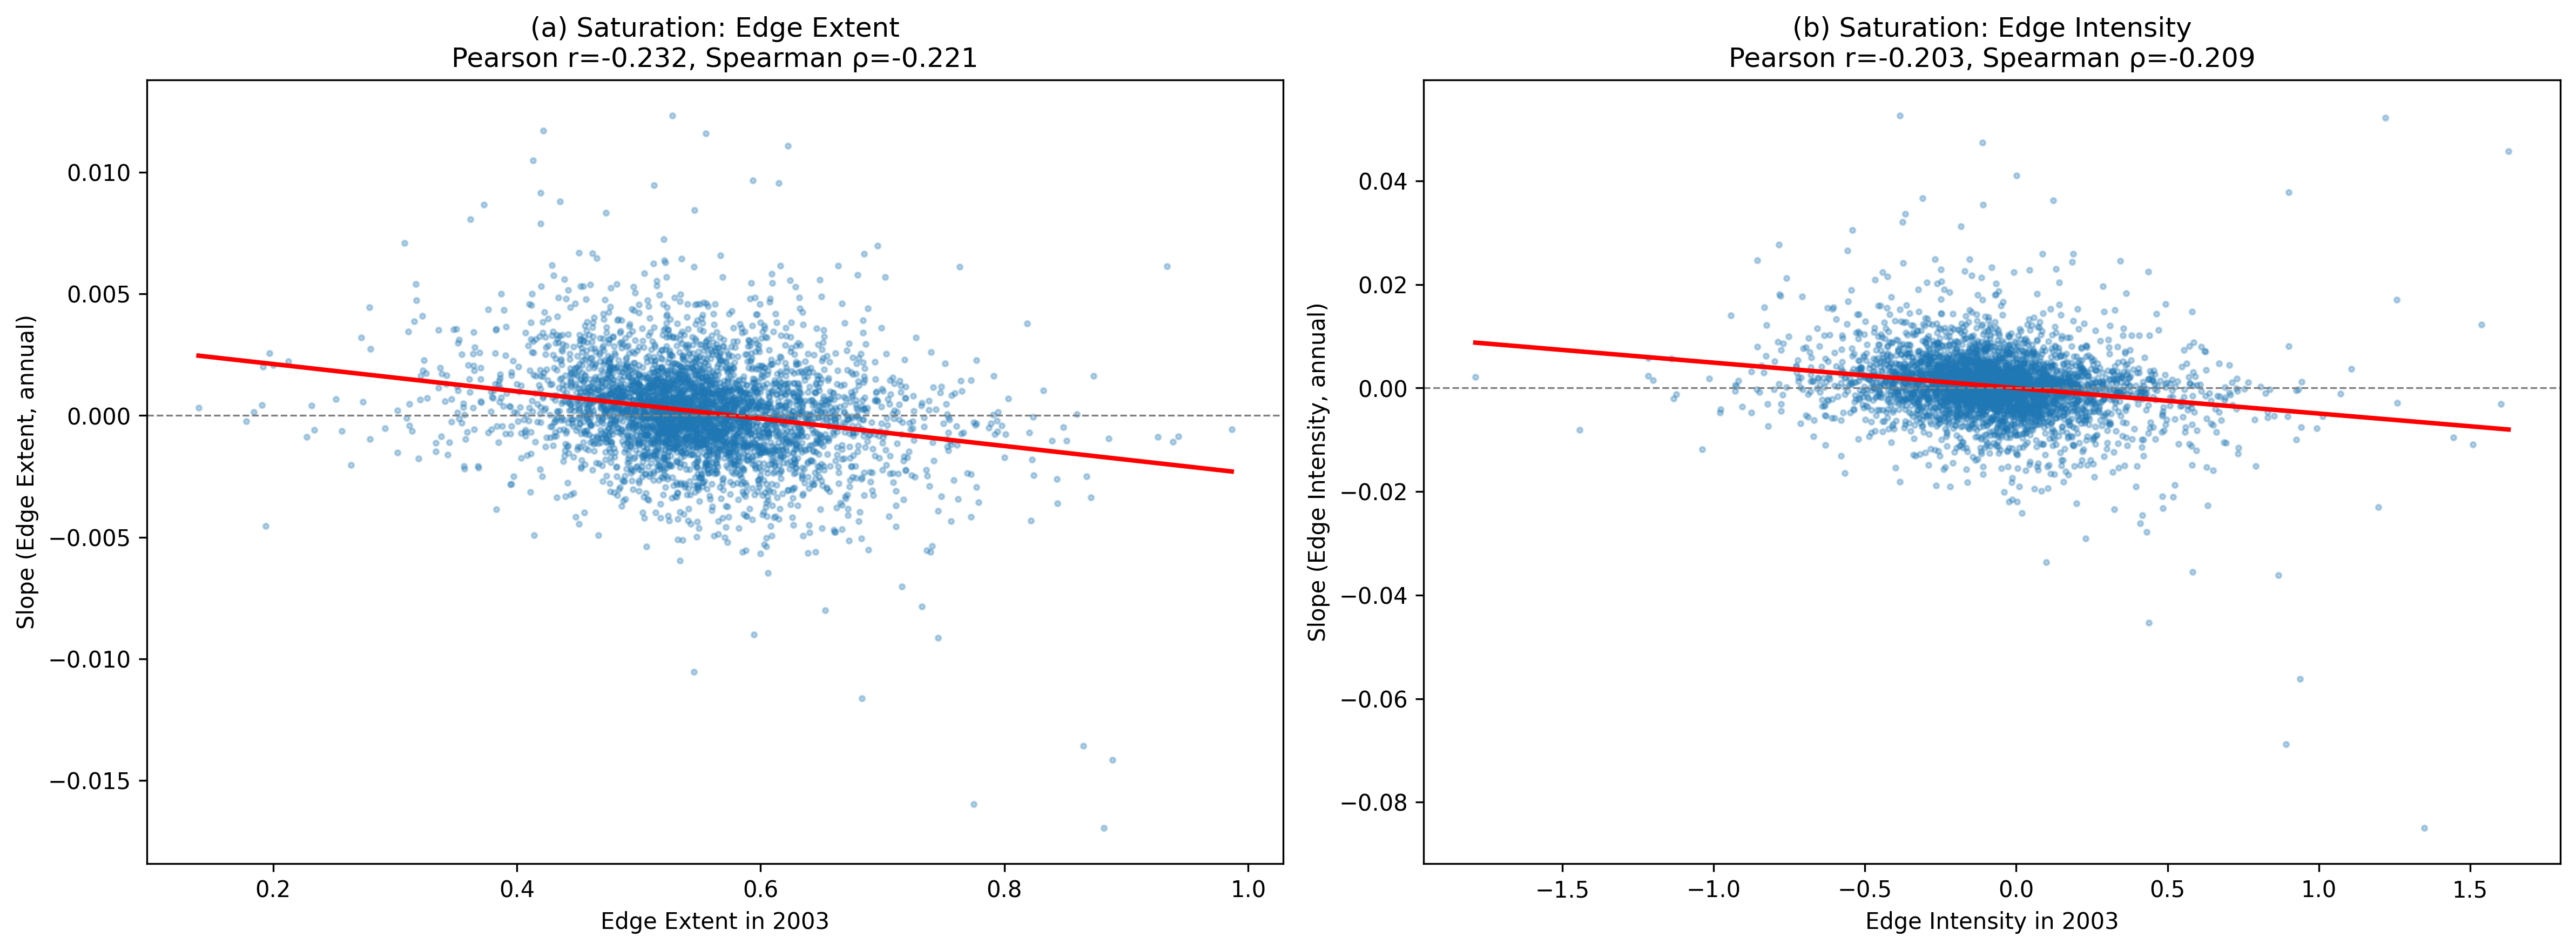
\includegraphics[width=1\linewidth]{files/ndvi_figure6_saturat-364ae31f0efe6b55eabccca22b496fe3.png}
\end{figure}


{\small \noindent \textbf{Figure 6.} (a) Saturation analysis for edge extent --- relationship between 2003 baseline and annual slope. (b) Same for edge intensity. Red lines show OLS fits.}

\vspace{1em}
PAs that already had high edge extent or intensity in 2003 tend to have lower or negative slopes, consistent with a saturation effect where boundaries with initially strong edges have limited capacity for further increase.

\begin{verbatim}
<IPython.core.display.Markdown object>
\end{verbatim}


\clearpage
\section{Supplementary Figures}

\begin{figure}[!htbp]
\centering
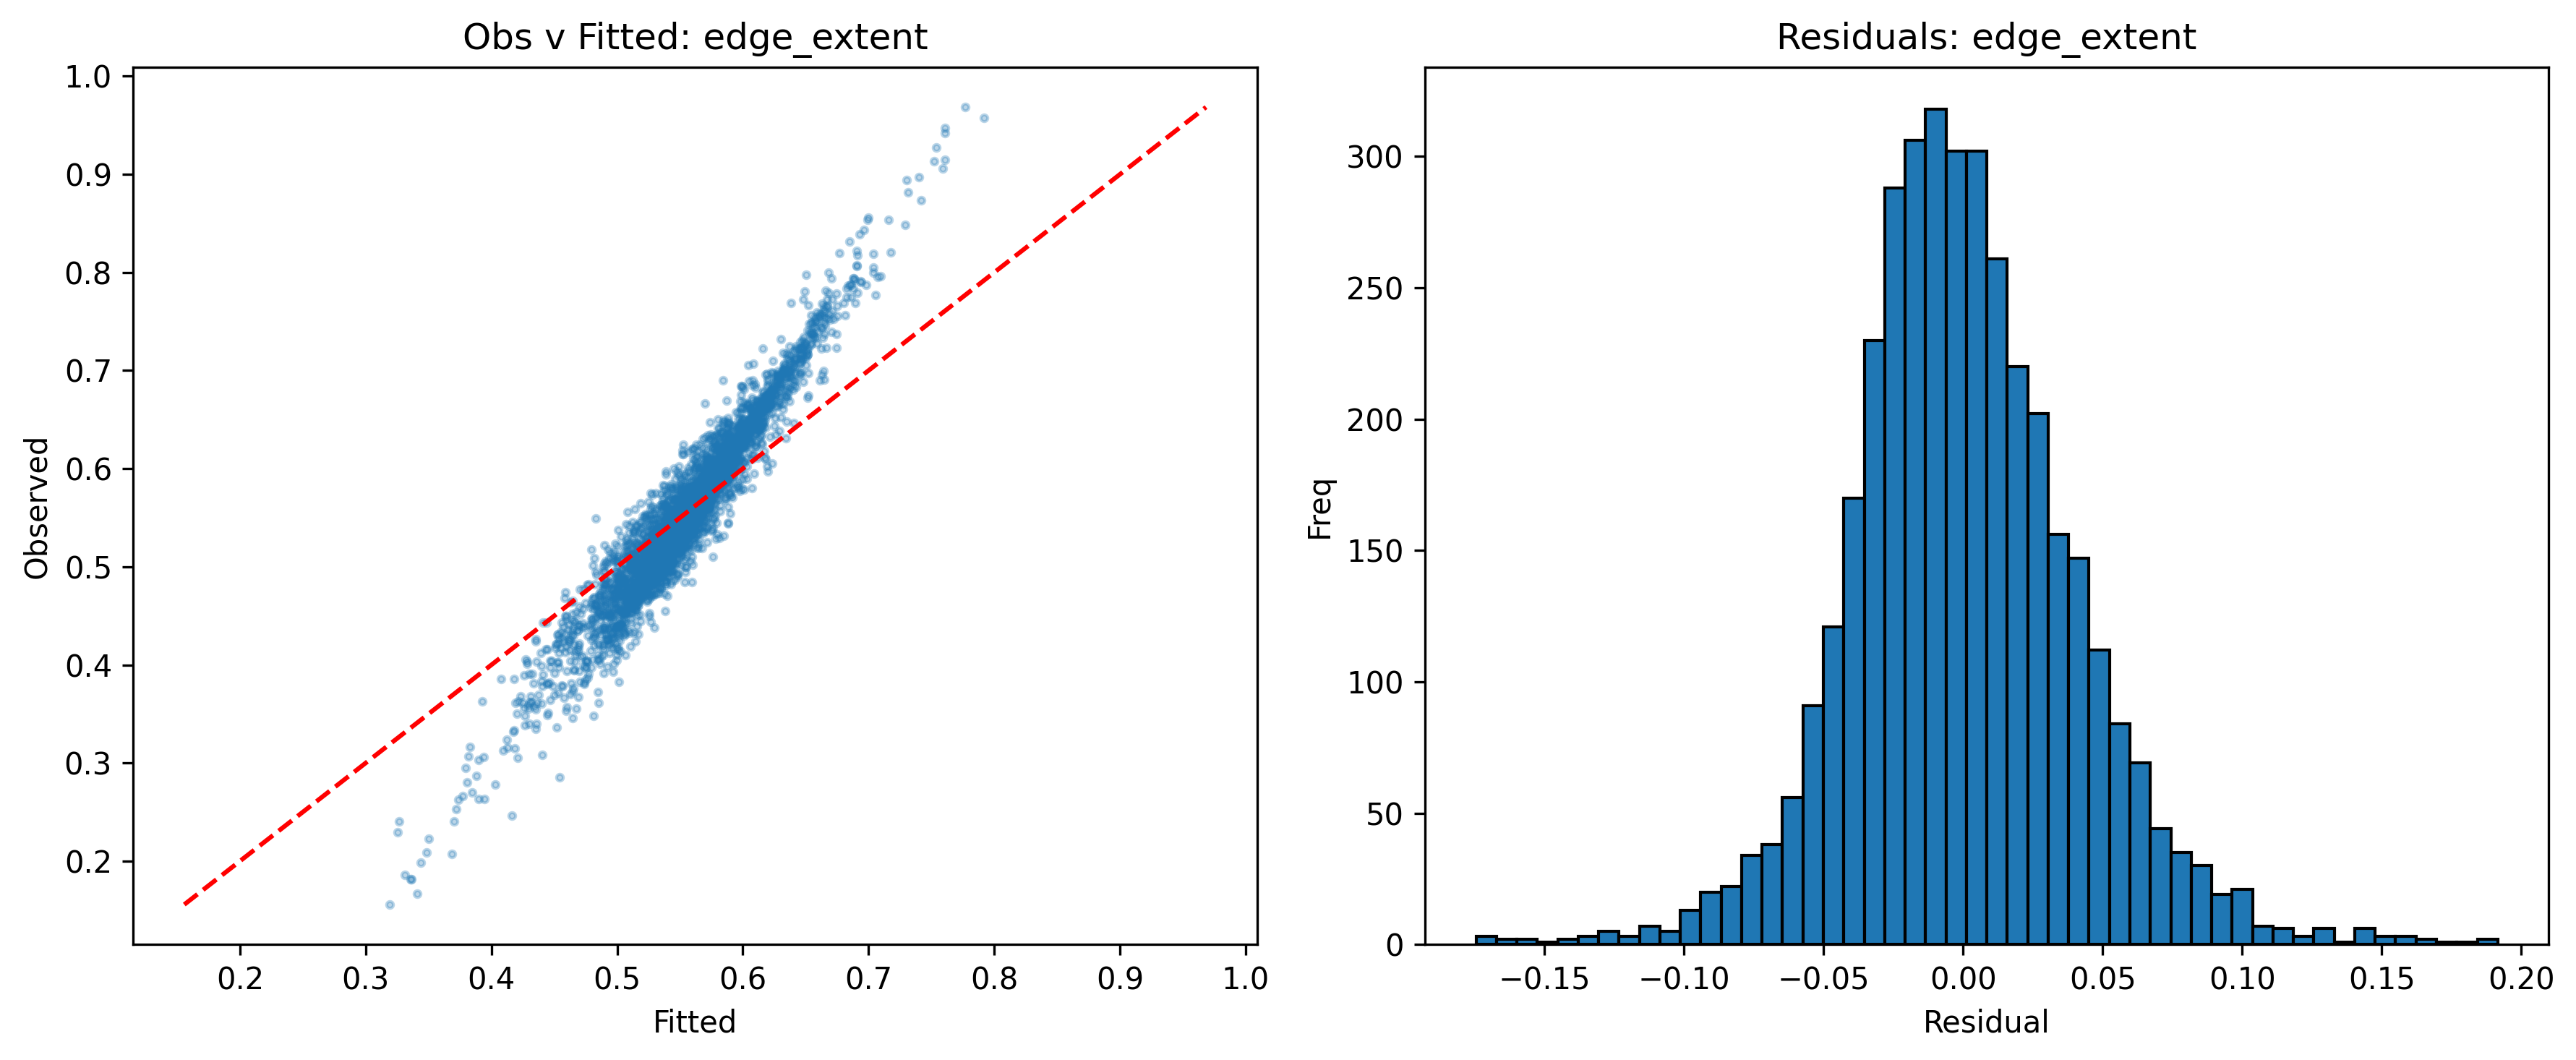
\includegraphics[width=1\linewidth]{files/ndvi_edge_extent_mod-d60c5d5bd604b108150788a9e354a3c8.png}
\end{figure}


{\small \noindent \textbf{Figure S1.} Diagnostics for the edge-extent mixed model: observed vs.\ fitted values (left) and residual distribution (right).}

\vspace{1em}
Residuals are approximately normally distributed and the observed-vs-fitted plot shows reasonable agreement, supporting model adequacy for edge extent.


\clearpage
\begin{figure}[!htbp]
\centering
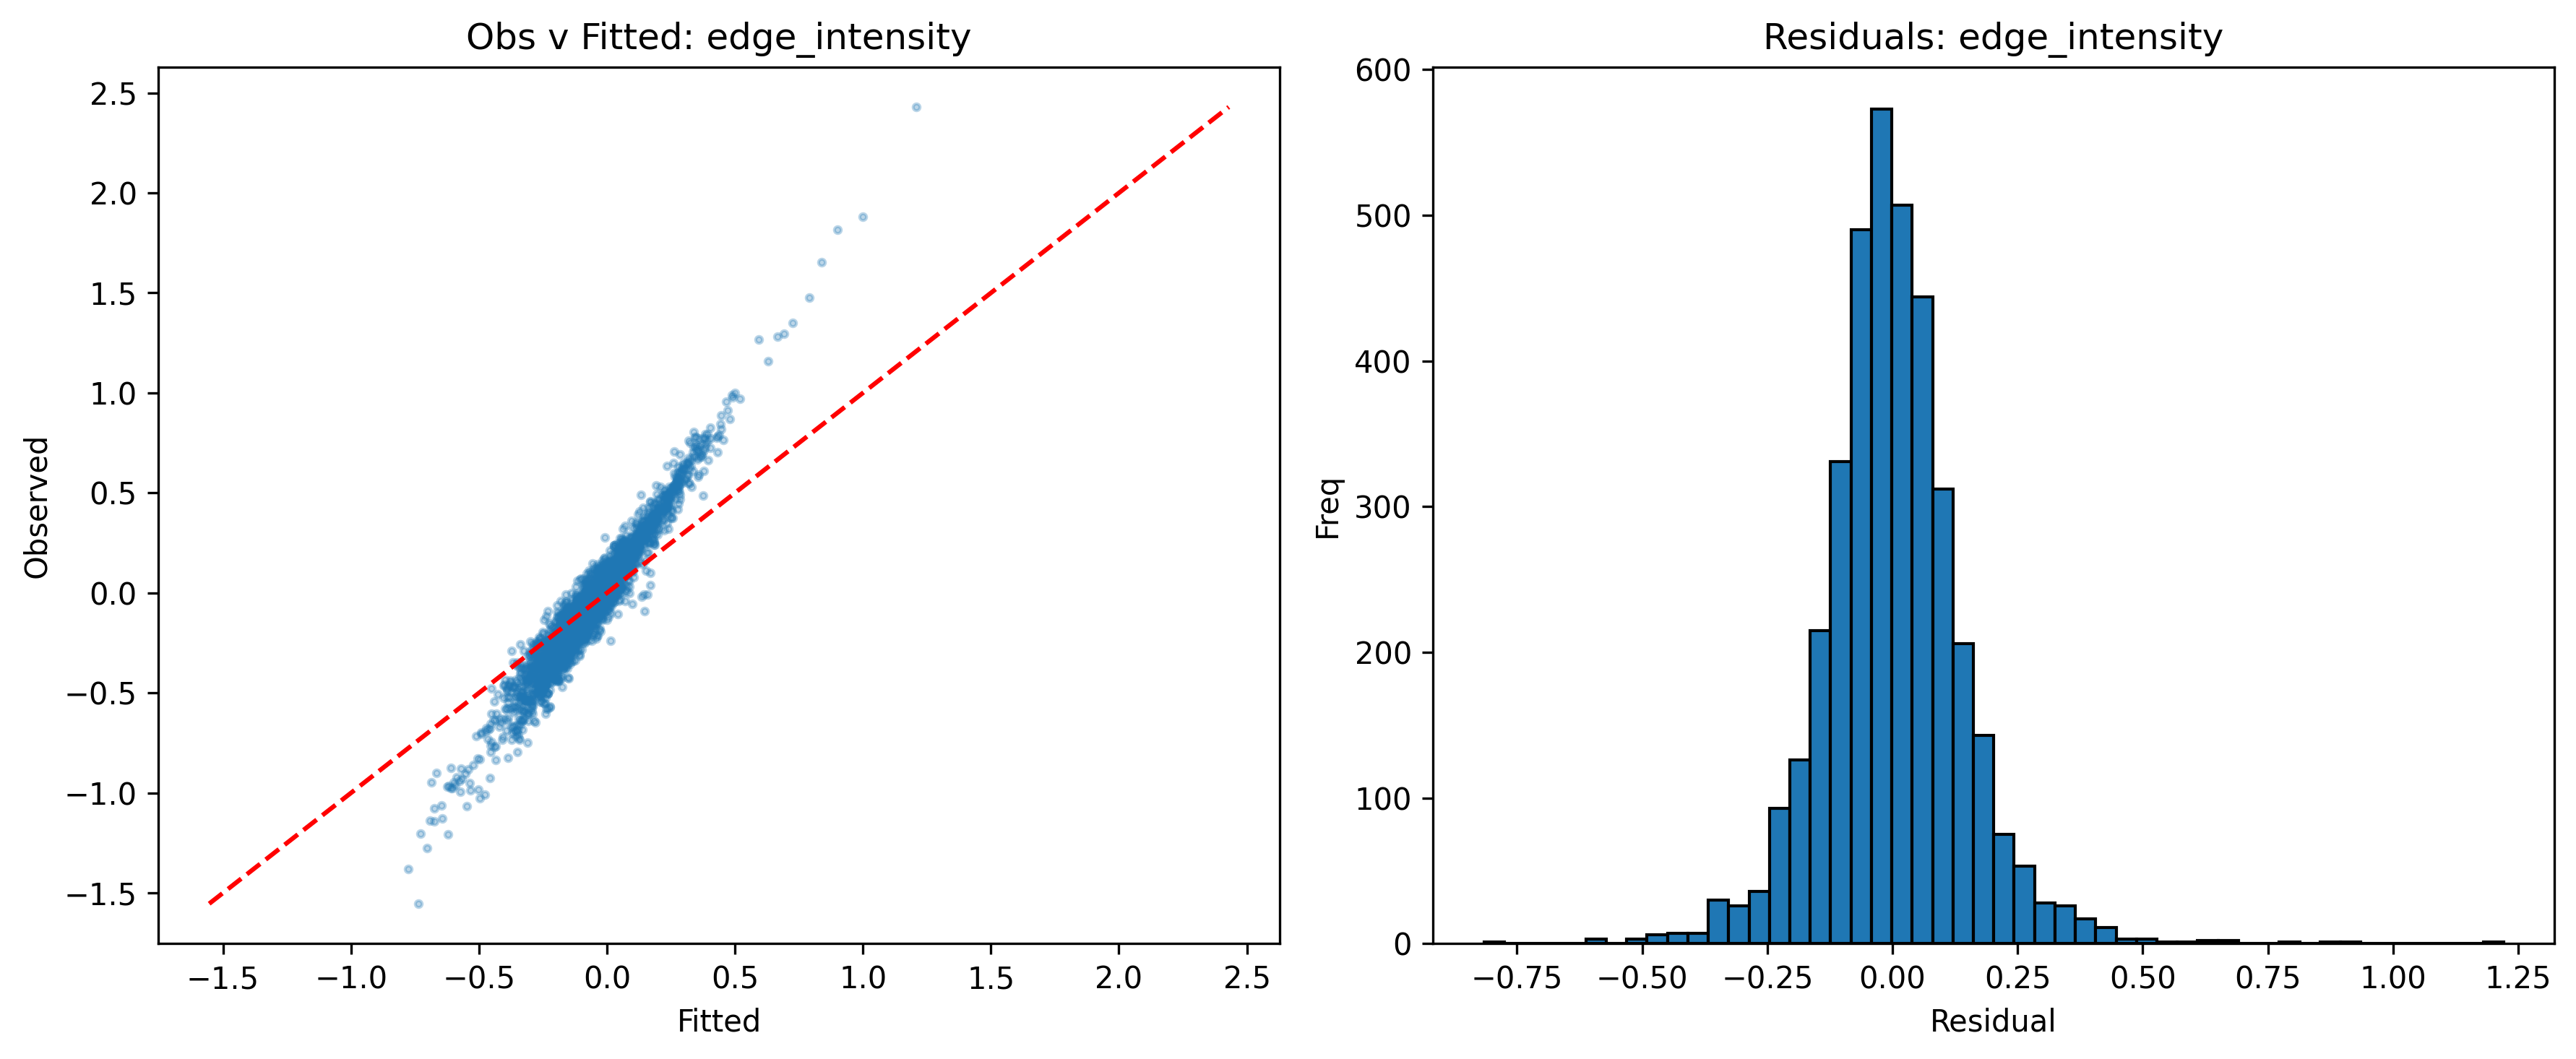
\includegraphics[width=1\linewidth]{files/ndvi_edge_intensity_-a7d21c57d6a4611d80ab7bd6211d5e55.png}
\end{figure}


{\small \noindent \textbf{Figure S2.} Diagnostics for the edge-intensity mixed model: observed vs.\ fitted values (left) and residual distribution (right).}

\vspace{1em}
The edge-intensity model shows greater residual spread, reflecting higher variability in Cohen's d across PAs, but residuals remain approximately symmetric.



\end{document}
